\documentclass{beamer}
\usetheme{Copenhagen}
\usecolortheme{seahorse}
\usefonttheme[onlymath]{serif}

\usepackage{setspace}
\usepackage{xcolor}
\usepackage{graphicx}
\usepackage{multimedia}
\usepackage{fontawesome5}
\usepackage[most]{tcolorbox}
\usepackage{empheq}
\usepackage{fancybox}
\usepackage{annotate-equations}
\usepackage{tikz}
\usetikzlibrary{positioning, calc, shapes.geometric, shapes.multipart, 
	shapes, arrows.meta, arrows, 
	decorations.markings, external, trees}
\tikzstyle{Arrow} = [
thick, 
decoration={
	markings,
	mark=at position 1 with {
		\arrow[thick]{latex}
	}
}, 
shorten >= 3pt, preaction = {decorate}
]

\definecolor{teel}{HTML}{00AEB3}
\definecolor{redorange}{HTML}{F26035}
\definecolor{ForestGreen}{RGB}{34,139,34}
\definecolor{darkgreen}{HTML}{06402B}
\definecolor{CarolinaBlue}{HTML}{4B9CD3}
\usecolortheme[named=CarolinaBlue]{structure}


\title[Addressing Positivity Violations]{Filling in the Blanks: Addressing Positivity Violations with Mathematical Models}
\author[Paul Zivich]{Paul Zivich \\~\\ Assistant Professor \\ Department of Epidemiology \\ Gillings School of Global Public Health \\ University of North Carolina at Chapel Hill}

\setbeamercovered{transparent}
\setbeamertemplate{navigation symbols}{}  % gets rid of the dumb navigation symbols
\setbeamertemplate{page number in head/foot}{\insertframenumber}  % adds slide #
\setbeamertemplate{headline}{}

\AtBeginSection[]{
	\begin{frame}
		\vfill
		\centering
		\begin{beamercolorbox}[sep=8pt,center,shadow=true,rounded=true]{title}
			\usebeamerfont{title}\insertsectionhead\par%
		\end{beamercolorbox}
		\vfill
	\end{frame}
}

\begin{document}
	
\begin{frame}[plain]
	\maketitle
\end{frame}

\begin{frame}{Acknowledgements\footnote[frame]{Footnotes are for asides or references}}
	\begin{center}
		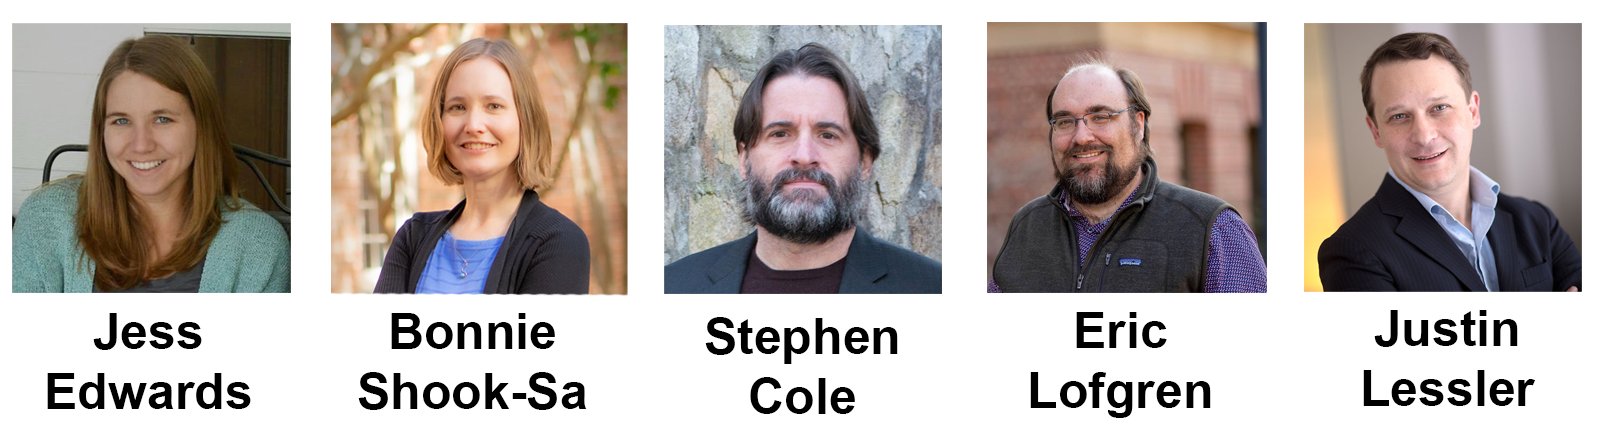
\includegraphics[width=0.90\linewidth]{images/coauthors.png}
	\end{center}
	\textbf{Publication}: arXiv:2503.02789 \\~\\
	\textbf{Funding}: K01AI177102, R01AI157758, P30AI050410 \\~\\
	\textbf{Disclaimer}: views are mine and not those of colleagues, NIH \\
	\begin{center}
		\small
		\faEnvelope \quad pzivich@unc.edu \qquad \quad 
		\faGithub \quad pzivich \qquad \quad
		\faHashtag \quad pausalz@bsky.social
	\end{center}
\end{frame}

\begin{frame}{Motivating Example}
	\textbf{Question}: What is the mean systolic blood pressure (SBP) in mm Hg among children and adolescents aged 2-17 in the United States?
	\\~\\~\\
	\textbf{Data}: NHANES 2017-2018
	\\~\\~\\
	\textbf{Challenge}: SBP is missing for 44\% children
\end{frame}

\begin{frame}{Notation}
	$Y$: systolic blood pressure (SBP) \\
	$R$: indicator if SBP was measured, with $1$ being yes \\
	$X$: a vector of covariates \\~\\
	$E[\cdot]$: expected value function \\
	$I(\cdot)$: indicator function, equal to $1$ when true, $0$ otherwise
	\\~\\
	\textbf{Parameter}: mean SBP if there was no missing data
	{\Large $$ \mu = E[Y] $$}
\end{frame}

\begin{frame}{Complete-Case Analysis}
	A complete-case analysis assumes
	{\Large $$ E[Y] = E[Y \mid R=1] $$}
	\begin{itemize}
		\item Missingness is independent of SBP (MCAR)
		\item Marginal exchangeability
	\end{itemize}
	~\\
	\begin{center}
		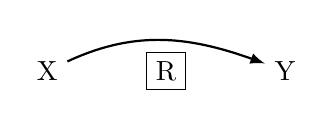
\begin{tikzpicture}
			\node  (1) {X};
			\node [right =of 1, rectangle, draw] (2) {R};
			\node [right =of 2] (3) {Y};
			
			%\draw[Arrow] (1.east) -- (2.west);
			\draw[Arrow] (1) to [out=25, in=160] (3); 
		\end{tikzpicture}
	\end{center}
	With extent of missingness, results are sensitive to assumption
\end{frame}

\begin{frame}{Addressing Missing Data}
	\textbf{Exchangeability}: SBP is missing at random conditional on age
	\begin{equation*}
		E[Y \mid X=x] = E[Y \mid X=x, R=1] \text{ for all values of } x
	\end{equation*}
	\begin{center}
		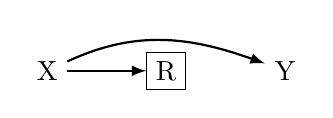
\begin{tikzpicture}
			\node  (1) {X};
			\node [right =of 1, rectangle, draw] (2) {R};
			\node [right =of 2] (3) {Y};
			
			\draw[Arrow] (1.east) -- (2.west);
			\draw[Arrow] (1) to [out=25, in=160] (3); 
		\end{tikzpicture}
	\end{center}
	~\\
	Under this assumption\footnote[frame]{Estimate with direct maximum likelihood estimator, g-computation}
	\begin{equation*}
		E[Y] = \sum_{x \in \mathcal{X}} E[Y \mid X=x, R=1] \Pr(X=x)
	\end{equation*}
	weighted average of the complete-case means within strata of $X$
\end{frame}

\begin{frame}{Positivity}
	For the previous exchangeability assumption, we need
	$$ \Pr(R=1 \mid X=x) > 0 \text{ for all values of } x $$
	~\\
	Every unique age has a non-zero probability of having $Y$ observed
	\begin{itemize}
		\item In the population
		\item Deterministic or structural positivity
	\end{itemize}
	%~\\
	%Not a statement about a particular sample $n$.\footnote[frame]{Zivich PN, Cole SR, \& Westreich D. (2022) \textit{arXiv:2207.05010}}
	%\begin{itemize}
	%	\item Could have bad luck
	%\end{itemize}
\end{frame}

%\begin{frame}{Positivity}
%	\begin{center}
%		
\includegraphics[width=0.9\linewidth]{images/missing-diagram1.png}
%	\end{center}
%\end{frame}

\begin{frame}{NHANES}
	In NHANES 2017-2018,
	\begin{itemize}
		\item ``BP is measured on participants 8 years and older"\footnote[frame]{\url{https://wwwn.cdc.gov/Nchs/Nhanes/2017-2018/BPX_J.htm}}
	\end{itemize}
	~\\~\\
	So $\Pr(R=1 \mid X=x) = 0$ for $x \in \{2,3,4,5,6,7\}$
	\begin{itemize}
		\item \textit{By design} of NHANES
	\end{itemize}
\end{frame}

%\begin{frame}{Nonpositivity}
%	\begin{center}
%		
\includegraphics[width=0.9\linewidth]{images/missing-diagram2.png}
%	\end{center}
%\end{frame}

\begin{frame}{NHANES Data}
	\begin{center}
		
\includegraphics[width=0.9\linewidth]{images/missing_nhanes1.png}
	\end{center}
\end{frame}

\begin{frame}{Options for Nonpositivity}
	\begin{itemize}
		\item[1.] Change parameter and question \\~\\
		\item[2.] Extrapolate from a statistical model \\~\\
		\item[3.] Synthesis of statistical and mathematical models
	\end{itemize}
\end{frame}

\begin{frame}{1. Change Parameter}
	\textbf{Parameter (revised)}: mean SBP for those 8 or older
	$$ E[Y \mid X \ge 8] $$
	~\\
	\textbf{Question}: what is the mean systolic blood pressure (SBP) in mm Hg among children and adolescents {\color{red} aged 8-17} in the US?
%	~\\~\\
%	\begin{center}
%		
\includegraphics[width=0.8\linewidth]{images/missing-diagram3.png}
%	\end{center}
\end{frame}

\begin{frame}{NHANES Data -- Restrict}
	\begin{center}
		
\includegraphics[width=0.9\linewidth]{images/missing_nhanes2.png}
	\end{center}
\end{frame}

\begin{frame}{2. Extrapolate}
	Fit a parametric model
	$$ E[Y \mid X \ge 8, R=1] = \beta_0 + \beta_1 X $$
	then back-fill missing SBP with model predictions
%	\begin{center}
%		
\includegraphics[width=0.9\linewidth]{images/missing-diagram4.png}
%	\end{center}
\end{frame}

\begin{frame}{NHANES Data -- Extrapolate}
	\begin{center}
		
\includegraphics[width=0.9\linewidth]{images/missing_nhanes3.png}
	\end{center}
\end{frame}

\begin{frame}{2. Extrapolate}
	Use of this model has two assumptions:
	\begin{itemize}
		\item[a.] Linear relationship with age for those 8-17 
		\item[b.] Linear relationship extends to those 2-7
	\end{itemize}
	~\\~\\
	(a) is in-principle checkable 
	\\~\\
	(b) is not checkable under nonpositivity
\end{frame}

\begin{frame}{3. Synthesis Modeling}
	Instead of extrapolating, integrate external information
	\begin{itemize}
		\item Address motivating question
		\item Avoid restrictive assumptions
	\end{itemize}
	~\\
	Divide parameter of interest in parts
	\\~\\
	\begin{equation*}
		\eqnmarkbox[darkgreen]{node0}{E[Y]} = \eqnmarkbox[blue]{node1}{E[Y \mid X \ge 8]} \Pr(X \ge 8) + \eqnmarkbox[red]{node2}{E[Y \mid X < 8]} \Pr(X < 8)
	\end{equation*}
	\annotate[yshift=0.75em]{above,right}{node0}{Overall mean}	
	\annotate[yshift=-0.75em]{below,right}{node1}{Mean in positive region}	
	\annotate[yshift=0.75em]{above,left}{node2}{Mean in nonpositive region}	
\end{frame}

%\begin{frame}{3. Synthesis Modeling}
%	\begin{center}
%		
\includegraphics[width=0.9\linewidth]{images/missing-diagram5.png}
%	\end{center}
%\end{frame}

\begin{frame}{Statistical Model}
	Identification
	$$ {\color{blue} E[Y \mid X \ge 8]} = E[E(Y \mid X, R=1, X \ge 8) \mid X \ge 8] $$
	\\~\\
	Use a statistical model: $E[Y \mid X,R=1,X \ge 8]$.\footnote[frame]{The identification result is also why 1. Change Parameter works}
	\begin{itemize}
		\item Estimate using the observed data
		\item Apply g-computation
	\end{itemize}
\end{frame}

\begin{frame}{Mathematical Model}
	Identification  
	$$ {\color{red} E[Y \mid X < 8]} = \; ?$$
	\begin{itemize}
		\item Data provide no information
	\end{itemize}
	~\\
	Appeal to external information
	\begin{itemize}
		\item Bounds for continuous $Y$: $(-\infty, \infty)$
		\item Bounds for SBP: $[0, 370]$
	\end{itemize}
	~\\
	Assume that\footnote[frame]{Structure and variations in mathematical model are rich enough}
	$$ E[Y \mid X=x] \in \mathcal{M}_{\alpha,x} \text{ for all } 2 \le x < 8$$
\end{frame}

\begin{frame}{Mathematical Model}
	We can do better still
	\begin{itemize}
		\item Published distributions of SBP\footnote[frame]{Flynn et al. 2017 \textit{Pediatrics} 140(3):e20171904}
		\item `Fill-in' missing SBP for those 2-7
	\end{itemize}
	~\\
	\textbf{Estimation}: Monte Carlo Procedure
	\begin{itemize}
		\item Draw random SBP based on tables for each unit
		\begin{itemize}
			\item Normal distribution by age, gender, height
		\end{itemize}
		\item Compute mean then repeat
	\end{itemize}
\end{frame}

\begin{frame}{NHANES Data -- Synthesis}
	\begin{center}
		
\includegraphics[width=0.9\linewidth]{images/missing_nhanes4.png}
	\end{center}
\end{frame}

\begin{frame}{Results -- Mean SBP}
	\begin{center}
		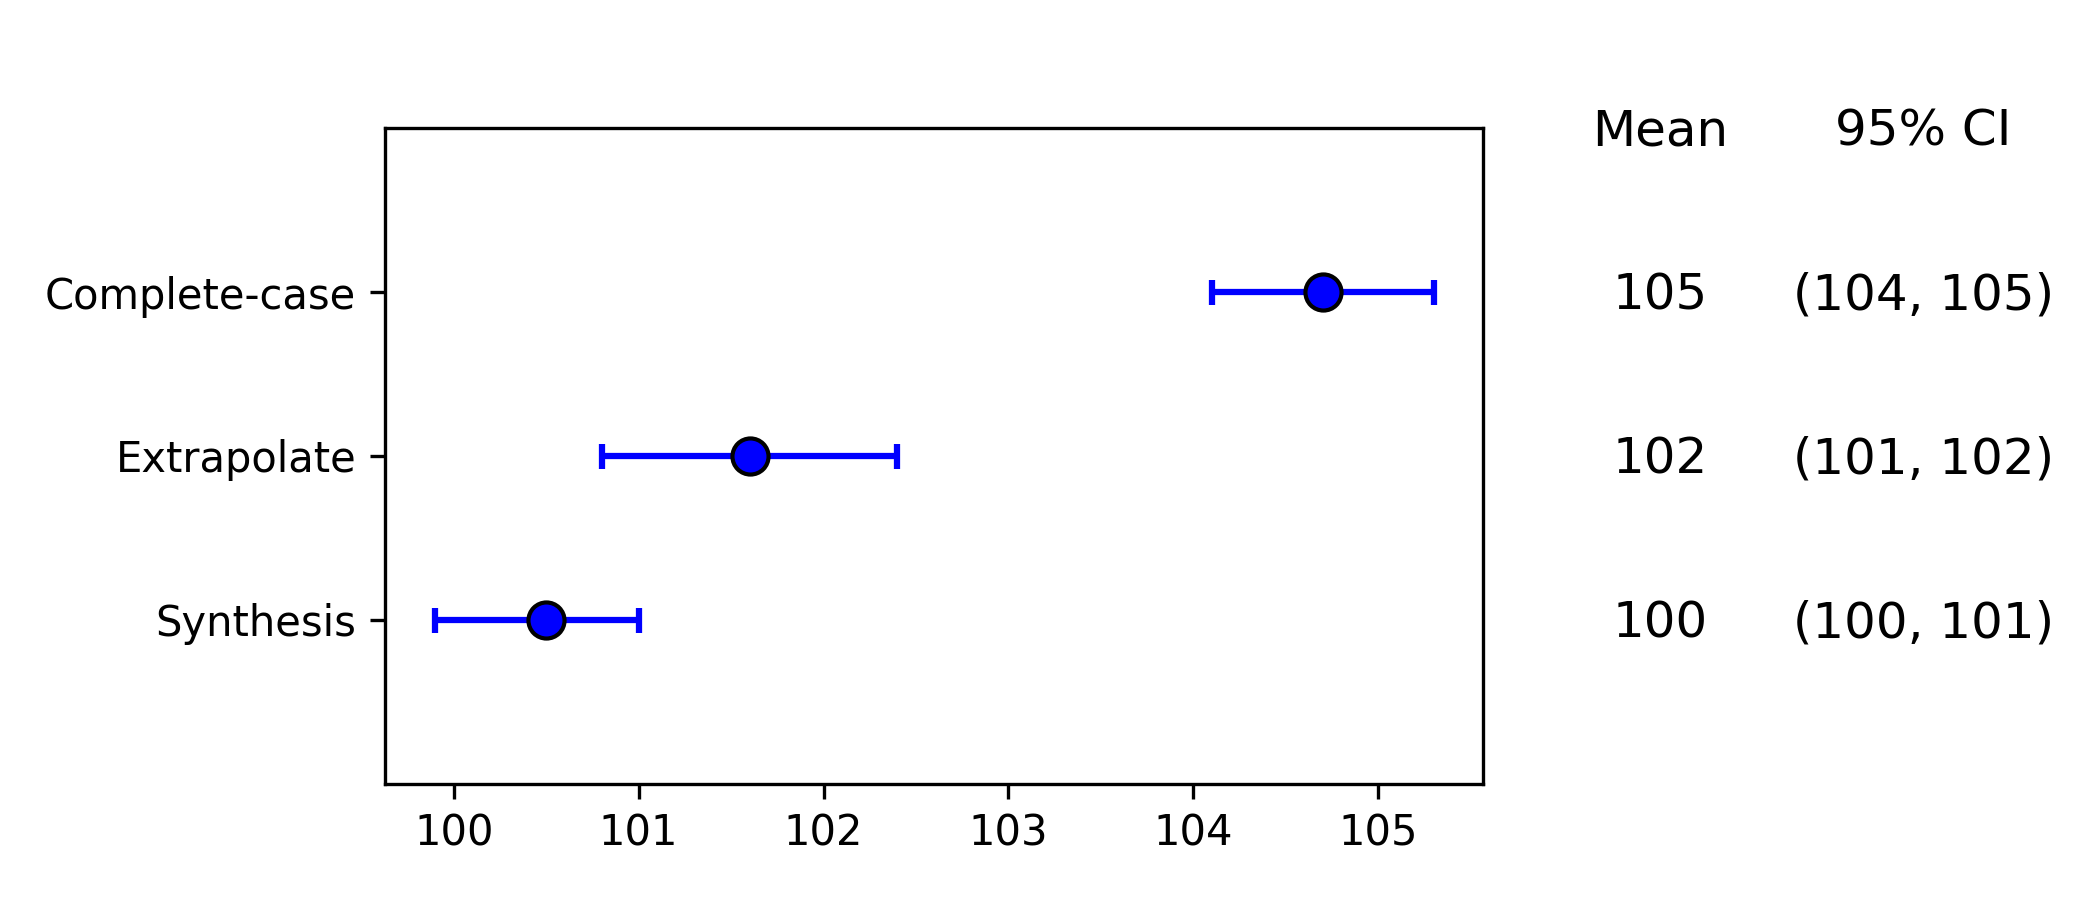
\includegraphics[width=0.9\linewidth]{images/nhanes_results.png}
	\end{center}
\end{frame}

\begin{frame}{Conclusion}
	Positivity is an important, but often unrecognized, assumption
	\begin{itemize}
		\item Appears with our exchangeability assumptions
	\end{itemize}
	~\\
	Synthesis of statistical and mathematical models to fill in missing data with nonpositivity
\end{frame}

\begin{frame}{Thank you}
	%\begin{center}
	%	{\Huge Questions?}
	%\end{center}
	%~\\
	\begin{center}
		\small
		\faEnvelope \quad pzivich@unc.edu \qquad \quad 
		\faGithub \quad pzivich \qquad \quad
		\faHashtag \quad pausalz@bsky.social
	\end{center}
	~\\
	Corresponding Publications
	\begin{itemize}
		\item Zivich et al. \textit{Epidemiology} 2024;35(1):23-31
		\item Zivich et al. \textit{JRSSA} 2025;188(1):158-180
		\item Zivich et al. \textit{arXiv:2503.02789}
	\end{itemize}
\end{frame}

\section{Appendix}

\begin{frame}{Why Positivity}
	\textbf{Intuition}: need some with $X=x$ to have $Y$ observed at least sometimes so can `stand-in' for without $Y$ measured
	\\~\\
	\textbf{Formally}: note that
	$$ E[Y \mid X=x, R=1] = \frac{E[Y R \; I(X=x)]}{\Pr(R=1 \mid X=x) \Pr(X=x)}$$
	with positivity preventing division by zero
	\\~\\~\\
	So, \textit{positivity} comes along with \textit{exchangeability}
\end{frame}


\end{document}